\documentclass[runningheads]{llncs}

\usepackage{graphicx}
\usepackage{booktabs}
\usepackage{multirow}
\usepackage{array}
\usepackage{amsmath}
\usepackage{url}

\begin{document}

\title{Securing Federated TinyML Intrusion Detection for IoT/MQTT Networks with ASCON-128 in an Edge--Fog--Cloud Architecture}
\titlerunning{Securing Federated TinyML IDS for IoT/MQTT Networks}

\author{Anonymous Authors}
\authorrunning{Anonymous Authors}
\institute{Anonymous Institution}

\maketitle

\begin{abstract}
IoT and Industrial IoT deployments increasingly rely on lightweight protocols such as MQTT, but intrusion detection in this setting remains constrained by limited memory, intermittent connectivity, and the privacy cost of centralizing traffic traces. This paper presents an Edge--Fog--Cloud intrusion detection system for IoT/MQTT networks that combines TinyML inference on ESP32-S3 nodes, local training on Raspberry Pi 4 gateways, hierarchical federated learning with FedAvg, and ASCON-128 authenticated encryption for the federated communication cycle. The system is evaluated on three traffic classes: \texttt{normal}, \texttt{mqtt\_bruteforce}, and \texttt{scan\_A}, represented by 13 unidirectional flow features. Eight experimental variants are compared: RN/MLP and CNN-1D models, each under ASCON and PLAIN communication, with and without Fog pre-aggregation. Across 56 global run summaries and 82,396 transport events, the best configuration, CNN-1D with ASCON and Fog, reached 0.975 final global accuracy and 0.091 loss in the evaluated MQTT scenario. ASCON-128 increased payload size and processing latency, but its p95 processing latency remained below 42.11 ms in the evaluated encrypted configurations. The results show that a protected federated TinyML IDS can be executed on a real IoT testbed, while also exposing limits related to heuristic labeling, restricted attack coverage, and the absence of Byzantine-robust aggregation.
\keywords{IoT security \and MQTT \and TinyML \and Hierarchical federated learning \and ASCON-128 \and Intrusion detection}
\end{abstract}

\section{Introduction}

IoT networks connect sensors, actuators, gateways, and cloud services under tight operational constraints. In domestic, laboratory, and industrial deployments, devices often use lightweight protocols, operate with limited compute resources, and produce traffic that varies across locations and use cases. MQTT is a common example: it is simple enough for constrained nodes, but its deployment in unattended or weakly monitored networks also expands the attack surface for brute-force attempts, scans, and misuse of exposed brokers.

Machine-learning-based network intrusion detection systems (NIDS) have reported strong classification performance in controlled datasets. However, a high offline score does not automatically imply a deployable IoT system. A practical IDS must execute close to the traffic source, limit communication, adapt to local traffic, and protect the messages exchanged during the learning process. These requirements create a gap between conventional centralized training pipelines and the constraints of microcontroller-based nodes.

This paper addresses that gap through an experimental system that integrates three components usually studied in isolation: TinyML-based inference, hierarchical federated learning (HFL), and lightweight authenticated encryption. The proposed testbed uses ESP32-S3 nodes at the Edge, Raspberry Pi 4 gateways at the Fog layer, and a PC coordinator at the Cloud layer. Edge nodes compute 13 flow features and run local inference. Gateways receive encrypted MQTT messages, label samples with a deterministic heuristic, train a compact neural model locally, and send only the federated layers to the PC. The coordinator applies FedAvg and redistributes the global model. ASCON-128 protects both MQTT and HTTP messages in the encrypted variants.

The central research question is not whether this IDS outperforms all existing classifiers. The question is narrower and more relevant for applied informatics: can a protected federated TinyML IDS be executed and measured on real IoT hardware while keeping the design small enough for edge deployment? To answer this, the system compares eight variants across model family, security mode, and aggregation topology.

The contributions are:
\begin{itemize}
    \item an Edge--Fog--Cloud IDS architecture for MQTT traffic using ESP32-S3, Raspberry Pi 4 gateways, and a PC coordinator;
    \item a lightweight federated TinyML pipeline where the Edge performs inference and gateways train the final MLP/RN or CNN-1D layers under FedAvg;
    \item an ASCON-128 protected federated cycle with measured latency and payload overhead against a PLAIN baseline;
    \item an experimental comparison of RN/MLP and CNN-1D models under ASCON/PLAIN and Fog/NoFog configurations.
\end{itemize}

\section{Related Work}

\subsection{IDS and TinyML for IoT}

IoT intrusion detection requires more than classification accuracy. A deployable model must fit the memory available in the node, respond within acceptable latency, and avoid excessive energy and communication costs. Recent TinyML-oriented IDS work has stressed that evaluation should report resource and execution metrics alongside accuracy \cite{Tekin2023_OnDeviceEnergy,Alwaisi2024,Amuthadevi2025,HeydariMahmoud2025_TinyML_IDS}. Broader surveys on IoT and IIoT security also show that many pipelines still depend on server-side training and evaluation, with limited validation on real microcontrollers \cite{Amanullah2020_DL_BigData_IoT_Security,Ni2024_IIoT_Security_Survey}.

Dini et al. review embedded AI for IIoT and discuss the toolchains used to deploy models on constrained platforms, including TensorFlow Lite Micro, STM32Cube.AI, and Vitis AI \cite{Dini2024_EmbeddedIIoT_Review}. Their analysis is relevant because deployment is not a final mechanical step; the model, feature representation, runtime, and hardware target must be considered together. This paper follows that perspective by treating inference, communication, local training, and security as part of one system.

\subsection{Federated Learning for IoT Security}

Federated learning reduces the need to centralize data by exchanging model updates instead of raw traces. In IoT security, this is useful because traffic flows can reveal device identities, services, and usage patterns. FL also introduces costs: clients may produce non-IID data, gateways may participate irregularly, and communication may dominate the cycle when messages are frequent or large \cite{Imteaj2022_FL_ResourceConstrainedSurvey,Albanbay2025}.

Recent FL-based IDS studies show this trade-off. Hajj et al. present a cross-layer federated IDS for IoT, and Roy et al. study adapted federated models under constrained settings \cite{Hajj2023_CrossLayerFL_IDS,Roy2023_FL_AdaptedModel}. Chaurasia et al. evaluate residual networks as FL clients in IIoT \cite{Chaurasia2024_FL_ResNet_IIoT}. Ficco et al. combine FL and transfer learning for on-board training on MCUs and Raspberry Pi 3 \cite{Ficco2024_FL_TinyML_Onboard}. These works motivate distributed learning, but deployment details differ across hardware, model size, and communication assumptions. In the present system, the ESP32-S3 performs inference and feature publication, while training is moved to Raspberry Pi 4 gateways.

\subsection{Lightweight Cryptography}

FL avoids moving raw data, but it does not make the training cycle automatically secure. Model weights, local metrics, and control messages are still sensitive. A gateway that receives corrupted global weights may update its local model incorrectly, and a server that accepts modified local weights may degrade the global model. For constrained systems, the protection mechanism must provide confidentiality and integrity without assuming a heavy cryptographic stack.

ASCON was selected by NIST as the basis for lightweight cryptography standards for constrained devices \cite{NISTSP8002322025}. Kaur et al. summarize ASCON implementations, differential and side-channel attacks, fault injection risks, and countermeasures \cite{Kaur2025_ASCON_Survey}. Other work has shown that ultra-lightweight ad-hoc permutation protocols for RFID/IoT can be broken experimentally on hardware \cite{Mirzaali2025_LWC_Permutations}. These results support using a standardized AEAD construction instead of custom XOR/rotation schemes. This paper uses ASCON-128 to protect the MQTT and HTTP payloads exchanged during the federated cycle.

\subsection{Positioning}

Table~\ref{tab:related_positioning} summarizes how the present work is positioned with respect to representative literature. The comparison is not intended to rank prior work. Its purpose is to clarify the integration gap addressed here. Several studies cover TinyML-based IDS, FL-based IDS, or lightweight cryptography for IoT. Fewer works evaluate the three elements together on a real Edge--Fog--Cloud testbed with microcontroller inference, gateway-side training, a cloud coordinator, and an explicit encrypted/plain baseline.

\begin{table}[t]
\centering
\caption{Positioning of this work against representative related work.}
\label{tab:related_positioning}
\begin{tabular}{p{0.25\linewidth}cccc}
\toprule
Work & TinyML IDS & FL/HFL & LWC/ASCON & Real multi-layer testbed \\
\midrule
TinyML IDS studies \cite{Tekin2023_OnDeviceEnergy,Amuthadevi2025,HeydariMahmoud2025_TinyML_IDS} & Yes & Limited & No & Limited \\
FL IDS for IoT \cite{Hajj2023_CrossLayerFL_IDS,Roy2023_FL_AdaptedModel,Chaurasia2024_FL_ResNet_IIoT} & Limited & Yes & No & Varies \\
FL + TinyML on-board \cite{Ficco2024_FL_TinyML_Onboard} & Yes & Yes & No & Yes \\
ASCON/LWC studies \cite{NISTSP8002322025,Kaur2025_ASCON_Survey,Mirzaali2025_LWC_Permutations} & No & No & Yes & Varies \\
This work & Yes & Yes & Yes & ESP32-S3, RPi 4, PC \\
\bottomrule
\end{tabular}
\end{table}

The proposed system is therefore framed as an experimental system paper. The novelty is not a new neural layer, a new FL optimizer, or a new cipher. The contribution is the joint implementation and measurement of these components in one applied IoT/MQTT security pipeline. This framing is important because the work studies whether a complete architecture can be assembled, instrumented, and evaluated under realistic hardware and communication constraints.

\section{System Architecture}

The proposed system follows a three-layer Edge--Fog--Cloud topology. Fig.~\ref{fig:architecture} summarizes the physical roles and data flow. The Edge layer contains ESP32-S3 nodes. Each node generates or observes MQTT-like flow events, extracts 13 numerical features, performs TinyML inference, and publishes encrypted feature vectors to the local gateway. The Fog layer is implemented with Raspberry Pi 4 gateways running Mosquitto, Python processing code, a local Keras model, and an HTTP endpoint. The Cloud layer is a PC running a FastAPI server that performs global aggregation and redistributes the federated model.

\begin{figure}[t]
\centering
\fbox{
\begin{minipage}{0.93\linewidth}
\centering
\textbf{Edge: ESP32-S3 nodes}\\
Flow generation/observation $\rightarrow$ 13 features $\rightarrow$ TinyML inference $\rightarrow$ MQTT publish\\[0.6em]
$\Downarrow$ ASCON-128 over MQTT (\texttt{fl/features}, \texttt{fl/global\_model})\\[0.6em]
\textbf{Fog: Raspberry Pi 4 gateways}\\
Mosquitto broker $\rightarrow$ ASCON verification $\rightarrow$ heuristic labeling $\rightarrow$ local Keras training\\[0.6em]
$\Downarrow$ ASCON-128 over HTTP (\texttt{/aggregate-from-gateway}, \texttt{/deploy-model})\\[0.6em]
\textbf{Cloud: PC coordinator}\\
FastAPI server $\rightarrow$ weighted FedAvg $\rightarrow$ model history dashboard $\rightarrow$ global model redistribution
\end{minipage}}
\caption{Logical architecture of the proposed HFL IDS. The Fog extension adds gateway-to-gateway communication before reporting a pre-aggregated update to the Cloud coordinator.}
\label{fig:architecture}
\end{figure}

The standard mode connects each gateway directly to the PC coordinator. The Fog mode adds gateway-to-gateway communication. In that mode, a leader gateway receives updates from a peer gateway, applies an intermediate FedAvg step, and sends a pre-aggregated update to the PC. This does not implement Byzantine consensus or blockchain. Its purpose is to measure whether an intermediate Fog aggregation layer changes convergence, round duration, and communication cost in the evaluated testbed.

The architecture uses two communication families. MQTT is used between ESP32-S3 nodes and Raspberry Pi 4 gateways. HTTP is used between gateways and the PC coordinator. In ASCON variants, messages are transmitted as JSON envelopes containing ciphertext (\texttt{ct}), authentication tag (\texttt{tag}), and nonce (\texttt{nonce}). In PLAIN variants, the same logical payloads are transmitted as JSON without encryption. This design makes the ASCON/PLAIN comparison functional rather than architectural: the same data path is preserved, while the security wrapper changes.

\section{Federated TinyML IDS Design}

\subsection{Flow Representation and Classes}

The IDS uses unidirectional flow features rather than raw packets or full PCAP traces. This choice reduces input size and makes the representation suitable for microcontroller-side processing. Each sample is represented by 13 features: number of packets, mean inter-arrival time, standard deviation of inter-arrival time, minimum and maximum inter-arrival time, mean packet length, total bytes, PSH flags, RST flags, URG flags, standard deviation of packet length, minimum packet length, and maximum packet length.

The evaluated classes are \texttt{normal}, \texttt{mqtt\_bruteforce}, and \texttt{scan\_A}. The data source contains 171,836 normal flows, 33,079 MQTT brute-force flows, and 51,358 scan flows, for 256,273 labeled rows after removing CSV headers. This class set is intentionally narrow. It represents a focused MQTT scenario rather than a complete taxonomy of IoT attacks.

\begin{table}[t]
\centering
\caption{Traffic classes and dataset rows used in the evaluated scenario.}
\label{tab:dataset}
\begin{tabular}{lrr}
\toprule
Class & Rows & Role in evaluation \\
\midrule
\texttt{normal} & 171,836 & Benign MQTT-like communication \\
\texttt{mqtt\_bruteforce} & 33,079 & Repeated MQTT login/connection attempts \\
\texttt{scan\_A} & 51,358 & Lightweight scanning behavior \\
\midrule
Total & 256,273 & Three-class IDS setting \\
\bottomrule
\end{tabular}
\end{table}

\subsection{Models}

The main model is a compact RN/MLP with topology $13 \rightarrow 32 \rightarrow 16 \rightarrow 8 \rightarrow 3$. The first two dense layers are kept fixed on the ESP32-S3 after initialization, while the final layers are federated. The exchanged parameters are $W_3$, $b_3$, $W_4$, and $b_4$, which keeps the federated payload small. This model has 1,139 parameters and is suitable for TinyML-style inference.

The second model family is a CNN-1D variant. It receives the same 13 features reshaped as a one-dimensional sequence. The convolutional part is used as a local feature extractor, and the final dense layers are included in the federated update. The CNN-1D branch is not introduced as a larger production model for the ESP32-S3; it is used to test whether a more expressive architecture improves the global behavior under the same communication protocol.

\subsection{Local Labeling and Training}

Gateways label incoming feature vectors using deterministic rules derived from the observed traffic statistics. A flow with many packets and many PSH flags is labeled as \texttt{mqtt\_bruteforce}. A short flow with small packets and few PSH flags is labeled as \texttt{scan\_A}. A flow with a small packet count and medium packet length is labeled as \texttt{normal}. Samples outside these rules are discarded. This design allows the system to run online without manual labels, but it is also a limitation because the local training signal depends on handcrafted thresholds.

For the experimental logs used in this paper, gateways trained on fixed local buffers recorded as 30 samples per update. Each local update used five epochs and mini-batches of eight samples. The current code branch should be checked before camera-ready submission because one inspected script sets the buffer target to 40 samples. The reported results in this paper follow the analyzed result logs, not the later code value.

\section{ASCON-128 Security Layer}

The ASCON layer protects the federated cycle at the message level. On ESP32-S3, features are serialized as JSON, encrypted with ASCON-128, and sent to the gateway through MQTT. The gateway decodes the envelope, verifies the tag, and rejects the message if authentication fails. For model updates, the gateway serializes the federated layers and local metrics, encrypts the payload, and posts it to the PC. The PC performs the same verification before including the update in FedAvg. The global model is then encrypted and sent back to the gateways, which forward it to the ESP32-S3 nodes.

ASCON is evaluated here as a communication security mechanism, not as a learning algorithm. Therefore, the expected effect is not an intrinsic increase in accuracy. The relevant measurements are latency, payload expansion, and whether the protected cycle still completes without disrupting convergence. This distinction is important: if encrypted variants show higher final accuracy in some runs, the result should be interpreted as an empirical behavior of the testbed and message filtering, not as a mathematical property of ASCON.

\section{Experimental Setup}

\subsection{Hardware and Software}

The testbed uses ESP32-S3 nodes for Edge inference, Raspberry Pi 4 gateways for local training and Fog aggregation, and a PC for the Cloud coordinator. The gateway layer runs Mosquitto for MQTT communication and Python code for decryption, labeling, local training, and HTTP communication. The PC runs a FastAPI server for receiving updates, applying FedAvg, recording metrics, and redistributing the global model.

The system was evaluated under eight variants, shown in Table~\ref{tab:variants}. The factor \emph{model} compares RN/MLP and CNN-1D. The factor \emph{security} compares ASCON-128 against PLAIN JSON. The factor \emph{topology} compares standard gateway-to-cloud aggregation against Fog pre-aggregation.

\begin{table}[t]
\centering
\caption{Experimental variants.}
\label{tab:variants}
\begin{tabular}{llll}
\toprule
Variant & Model & Security & Topology \\
\midrule
RN\_ASCON & RN/MLP & ASCON-128 & NoFog \\
RN\_PLAIN & RN/MLP & Plain JSON & NoFog \\
RN\_FOG\_ASCON & RN/MLP & ASCON-128 & Fog \\
RN\_FOG\_PLAIN & RN/MLP & Plain JSON & Fog \\
CNN\_ASCON & CNN-1D & ASCON-128 & NoFog \\
CNN\_PLAIN & CNN-1D & Plain JSON & NoFog \\
CNN\_FOG\_ASCON & CNN-1D & ASCON-128 & Fog \\
CNN\_FOG\_PLAIN & CNN-1D & Plain JSON & Fog \\
\bottomrule
\end{tabular}
\end{table}

\subsection{Metrics}

The evaluation records global accuracy, global loss, local training metrics, round duration, ASCON/PLAIN processing time, payload size, and message expansion ratio. The consolidated analysis includes eight configured experiments, 58 discovered attempts, 337 CSV files, 82,396 transport events, 2,648 model-metric rows, and 56 global attempt summaries. Timing summaries exclude a malformed negative round-duration row found in one RN Fog ASCON run. This exclusion affects timing aggregation only.

\section{Results and Discussion}

\subsection{Global Detection Performance}

Table~\ref{tab:global_results} summarizes the final global performance by variant. The strongest result was obtained by CNN-1D with ASCON and Fog, with 0.9750 final accuracy and 0.0910 loss. The CNN family outperformed the RN/MLP family in this scenario, especially under Fog aggregation. RN/MLP remained viable and compact, but its results were more sensitive to topology and security mode.

\begin{table}[t]
\centering
\caption{Global results by variant. Accuracy and loss are averages of final global values across available run summaries. Timing uses positive round-duration rows.}
\label{tab:global_results}
\begin{tabular}{llrrrr}
\toprule
Model & Variant & Summaries & Final acc. & Final loss & Avg. round (s) \\
\midrule
CNN-1D & ASCON + Fog & 6 & 0.9750 & 0.0910 & 58.61 \\
CNN-1D & ASCON + NoFog & 8 & 0.9604 & 0.1040 & 58.97 \\
CNN-1D & PLAIN + Fog & 3 & 0.9444 & 0.1190 & 54.86 \\
CNN-1D & PLAIN + NoFog & 3 & 0.9389 & 0.1363 & 52.02 \\
RN/MLP & ASCON + Fog & 5 & 0.9633 & 0.1124 & 71.50 \\
RN/MLP & ASCON + NoFog & 14 & 0.9381 & 0.1545 & 72.91 \\
RN/MLP & PLAIN + NoFog & 14 & 0.9298 & 0.1581 & 51.01 \\
RN/MLP & PLAIN + Fog & 3 & 0.9000 & 0.2199 & 67.14 \\
\bottomrule
\end{tabular}
\end{table}

The results support three observations. First, the architecture can complete repeated federated cycles with real hardware and encrypted communication. Second, ASCON did not prevent convergence in the evaluated configurations. Third, Fog aggregation helped the best CNN and RN ASCON variants, but it did not help all configurations. The RN PLAIN Fog case performed worse than its NoFog counterpart, which suggests that intermediate aggregation is not automatically beneficial. Its effect depends on model behavior, local data distributions, and timing.

\begin{figure}[t]
\centering

\includegraphics[width=0.96\linewidth]{figures/global_accuracy_loss.png}
\caption{Global accuracy and loss trends across the consolidated HFL experiments.}
\label{fig:acc_loss}
\end{figure}

\subsection{ASCON-128 Cost}

ASCON increased payload size because ciphertext, tag, and nonce are transmitted inside a JSON envelope. For small ESP32-to-gateway feature messages, this expansion is proportionally large. For model-weight messages, the relative expansion is lower because the plaintext payload is already several kilobytes. In the consolidated ASCON experiment summaries, average expansion ratios ranged from 1.85 to 1.93, and average overhead percentages ranged from 84.53\% to 93.31\%.

The p95 ASCON processing latency remained below 42.11 ms in all encrypted experiment groups. Edge feature-message decryption at the gateway showed p95 values around 4.25--4.73 ms. Larger gateway and server messages, especially global model redistribution and Fog peer communication, produced higher p95 values. These measurements are not negligible, but they are small compared with federated round durations measured in tens of seconds.

\begin{figure}[t]
\centering

\includegraphics[width=0.90\linewidth]{figures/transport_latency_p95.png}
\caption{p95 transport processing latency by channel and experiment. ASCON variants include encryption or decryption; PLAIN variants include serialization or deserialization.}
\label{fig:latency}
\end{figure}

\begin{figure}[t]
\centering
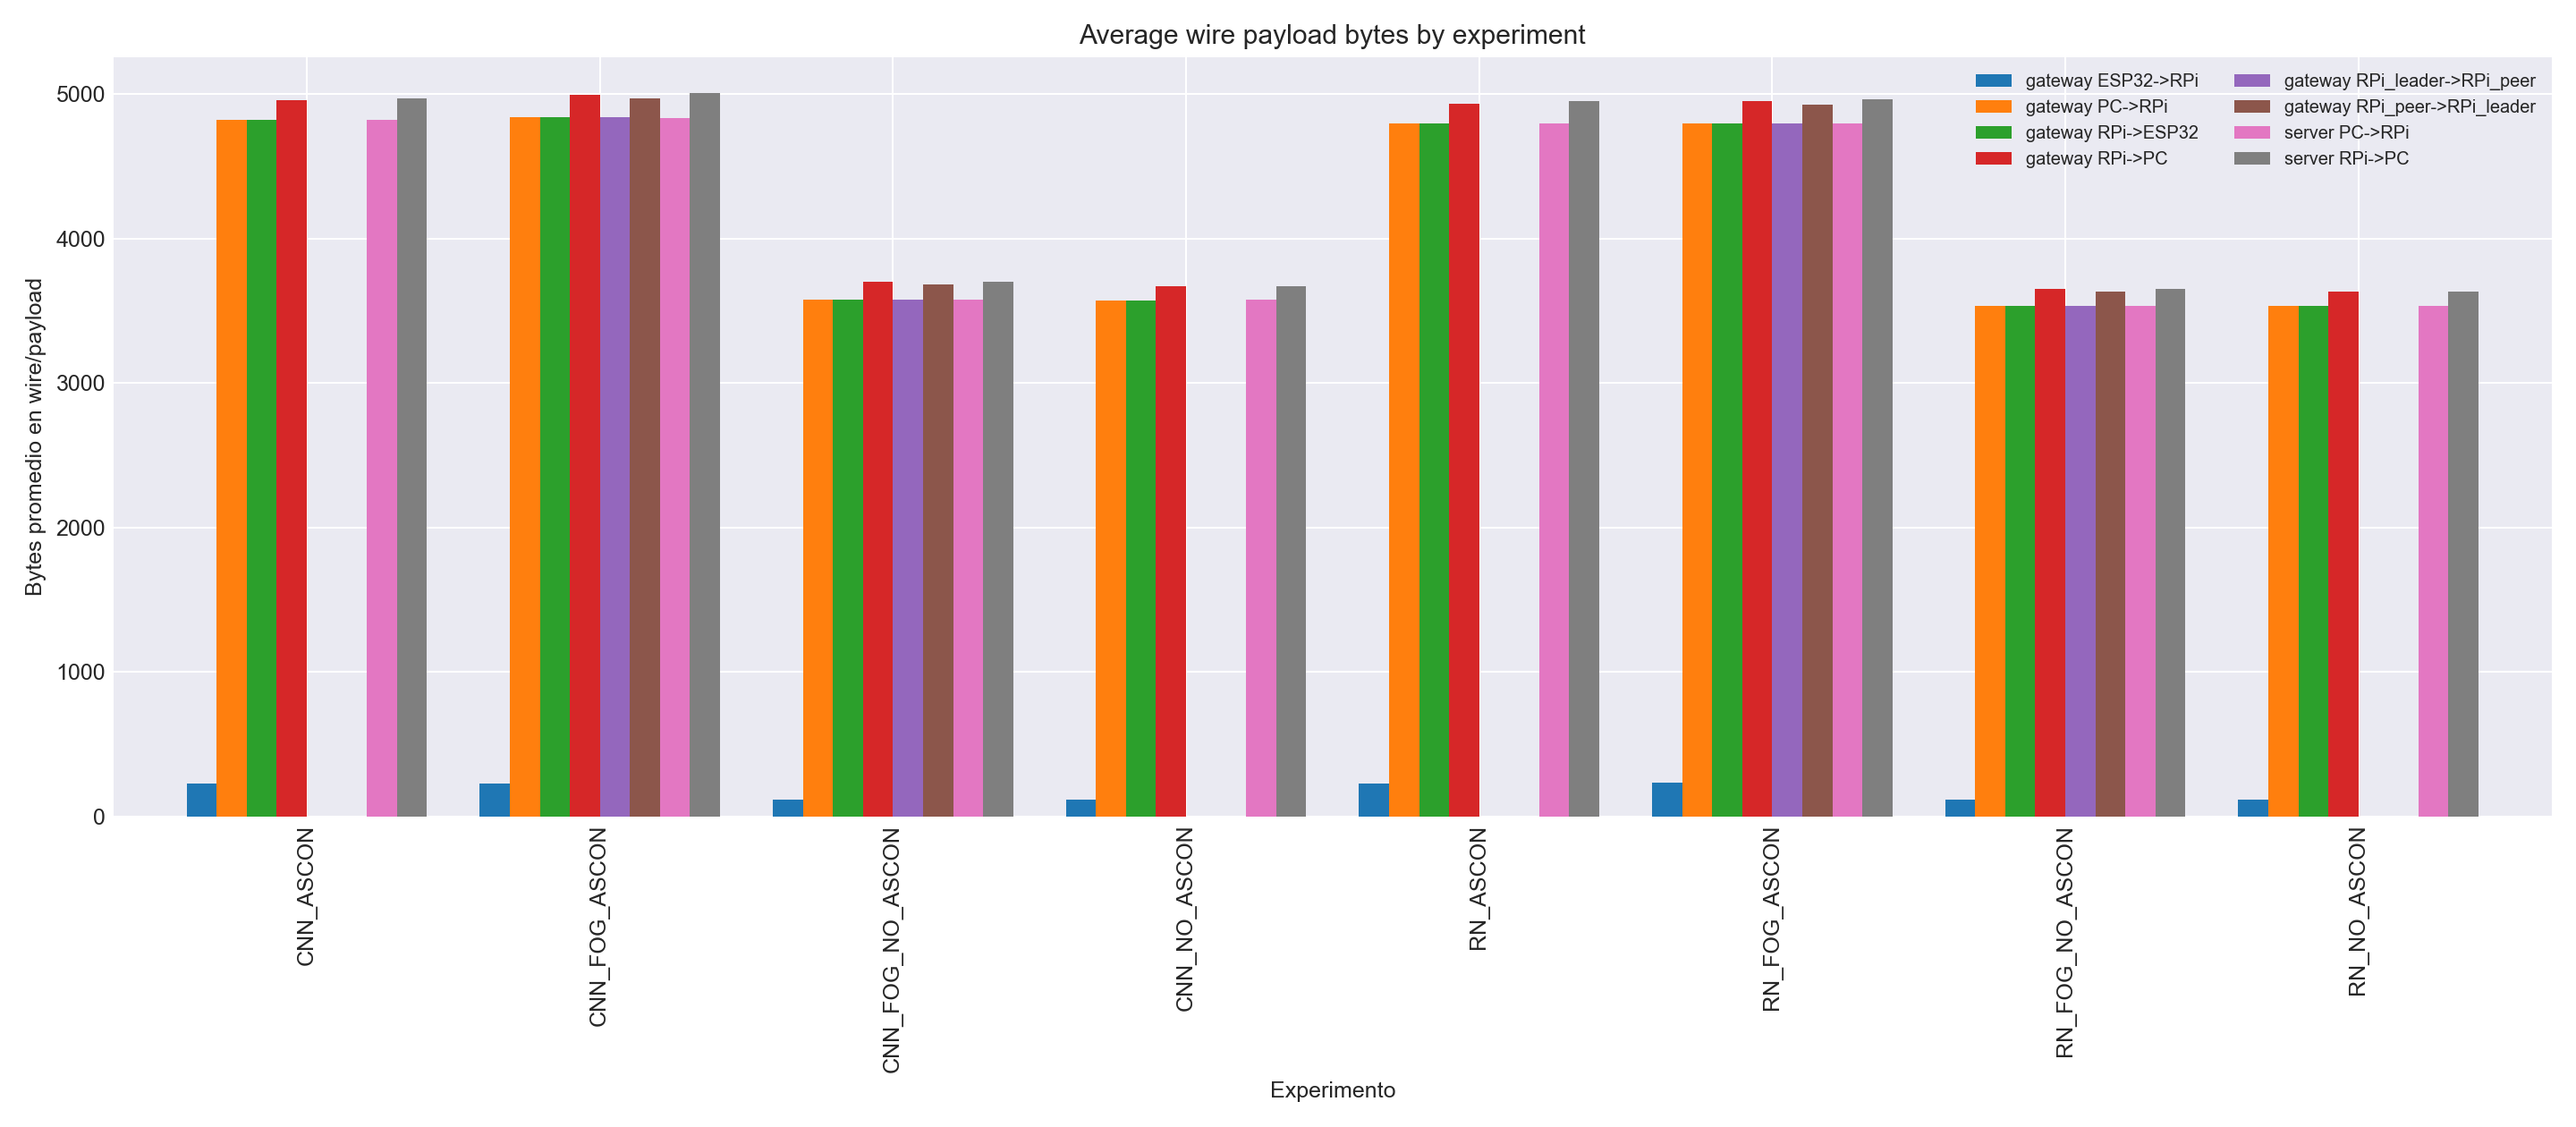
\includegraphics[width=0.90\linewidth]{figures/transport_payload_bytes.png}
\caption{Payload size comparison across transport channels. ASCON envelopes increase wire bytes because they carry ciphertext, tag, and nonce.}
\label{fig:payload}
\end{figure}

\subsection{Fog Aggregation}

Fog aggregation improved the best ASCON configurations: CNN ASCON improved from 0.9604 to 0.9750 final accuracy, and RN ASCON improved from 0.9381 to 0.9633. The same conclusion does not hold for all PLAIN cases. CNN PLAIN improved slightly with Fog, while RN PLAIN degraded. This result is useful because it avoids a simplistic claim that Fog is always better. The data suggest that Fog pre-aggregation can help, but only when the model and local update behavior are stable enough for the intermediate average to be beneficial.

\subsection{Model Choice}

The RN/MLP model is smaller and easier to deploy on the ESP32-S3. Its 1,139 parameters make it attractive for TinyML inference and fast local updates of the final layers. The CNN-1D variant performed better in the evaluated runs, but it is also more complex and should be evaluated more carefully before being treated as the default edge model. For a deployable IoT system, the best model is not necessarily the model with the highest accuracy; it is the model that preserves an acceptable balance among memory, latency, communication, and robustness.

\section{Threats to Validity}

The evaluation has several limits. First, only three classes were evaluated: \texttt{normal}, \texttt{mqtt\_bruteforce}, and \texttt{scan\_A}. This is a focused MQTT intrusion scenario, not a complete IDS benchmark. Second, the ESP32-S3 simulated or reproduced flow statistics derived from datasets; the study does not claim continuous live capture from a production network. Third, gateway labels are assigned through heuristics. This makes online experimentation feasible, but it also means that labeling errors can affect local training.

Fourth, the testbed uses a small number of gateways and does not establish large-scale FL behavior. Fifth, the system does not implement Byzantine-robust aggregation, poisoning detection, membership-inference defenses, or differential privacy. A compromised gateway could still send malicious weights to the coordinator. Sixth, ASCON side-channel resistance was not tested. The study measures message-level confidentiality and integrity under a controlled physical setting; it does not evaluate power analysis, electromagnetic leakage, or fault injection. Finally, energy consumption was not measured directly on the ESP32-S3, which should be addressed before claiming battery-oriented deployment.

\section{Conclusion}

This paper presented a first version of an Edge--Fog--Cloud IDS for IoT/MQTT networks that combines TinyML inference, hierarchical federated learning, and ASCON-128 message protection. The system was implemented on ESP32-S3 nodes, Raspberry Pi 4 gateways, and a PC coordinator. It compared RN/MLP and CNN-1D models across ASCON/PLAIN and Fog/NoFog configurations.

The best observed variant, CNN-1D with ASCON and Fog, reached 0.9750 final global accuracy and 0.0910 loss. ASCON-128 increased payload size and processing time, but p95 processing latency remained below 42.11 ms in the encrypted configurations analyzed. These results indicate that protected federated TinyML intrusion detection is feasible in the evaluated testbed. The main limitations are the narrow class set, heuristic labeling, small topology, and absence of adversarial FL defenses. Future work should evaluate real continuous traffic capture, larger gateway populations, energy consumption, Byzantine-robust aggregation, and side-channel-resistant ASCON implementations.

\bibliographystyle{splncs04}
\bibliography{references}

\end{document}
